\documentclass[twoside]{book}

% Packages required by doxygen
\usepackage{fixltx2e}
\usepackage{calc}
\usepackage{doxygen}
\usepackage[export]{adjustbox} % also loads graphicx
\usepackage{graphicx}
\usepackage[utf8]{inputenc}
\usepackage{makeidx}
\usepackage{multicol}
\usepackage{multirow}
\PassOptionsToPackage{warn}{textcomp}
\usepackage{textcomp}
\usepackage[nointegrals]{wasysym}
\usepackage[table]{xcolor}

% Font selection
\usepackage[T1]{fontenc}
\usepackage[scaled=.90]{helvet}
\usepackage{courier}
\usepackage{amssymb}
\usepackage{sectsty}
\renewcommand{\familydefault}{\sfdefault}
\allsectionsfont{%
  \fontseries{bc}\selectfont%
  \color{darkgray}%
}
\renewcommand{\DoxyLabelFont}{%
  \fontseries{bc}\selectfont%
  \color{darkgray}%
}
\newcommand{\+}{\discretionary{\mbox{\scriptsize$\hookleftarrow$}}{}{}}

% Page & text layout
\usepackage{geometry}
\geometry{%
  a4paper,%
  top=2.5cm,%
  bottom=2.5cm,%
  left=2.5cm,%
  right=2.5cm%
}
\tolerance=750
\hfuzz=15pt
\hbadness=750
\setlength{\emergencystretch}{15pt}
\setlength{\parindent}{0cm}
\setlength{\parskip}{3ex plus 2ex minus 2ex}
\makeatletter
\renewcommand{\paragraph}{%
  \@startsection{paragraph}{4}{0ex}{-1.0ex}{1.0ex}{%
    \normalfont\normalsize\bfseries\SS@parafont%
  }%
}
\renewcommand{\subparagraph}{%
  \@startsection{subparagraph}{5}{0ex}{-1.0ex}{1.0ex}{%
    \normalfont\normalsize\bfseries\SS@subparafont%
  }%
}
\makeatother

% Headers & footers
\usepackage{fancyhdr}
\pagestyle{fancyplain}
\fancyhead[LE]{\fancyplain{}{\bfseries\thepage}}
\fancyhead[CE]{\fancyplain{}{}}
\fancyhead[RE]{\fancyplain{}{\bfseries\leftmark}}
\fancyhead[LO]{\fancyplain{}{\bfseries\rightmark}}
\fancyhead[CO]{\fancyplain{}{}}
\fancyhead[RO]{\fancyplain{}{\bfseries\thepage}}
\fancyfoot[LE]{\fancyplain{}{}}
\fancyfoot[CE]{\fancyplain{}{}}
\fancyfoot[RE]{\fancyplain{}{\bfseries\scriptsize Generated by Doxygen }}
\fancyfoot[LO]{\fancyplain{}{\bfseries\scriptsize Generated by Doxygen }}
\fancyfoot[CO]{\fancyplain{}{}}
\fancyfoot[RO]{\fancyplain{}{}}
\renewcommand{\footrulewidth}{0.4pt}
\renewcommand{\chaptermark}[1]{%
  \markboth{#1}{}%
}
\renewcommand{\sectionmark}[1]{%
  \markright{\thesection\ #1}%
}

% Indices & bibliography
\usepackage{natbib}
\usepackage[titles]{tocloft}
\setcounter{tocdepth}{3}
\setcounter{secnumdepth}{5}
\makeindex

% Hyperlinks (required, but should be loaded last)
\usepackage{ifpdf}
\ifpdf
  \usepackage[pdftex,pagebackref=true]{hyperref}
\else
  \usepackage[ps2pdf,pagebackref=true]{hyperref}
\fi
\hypersetup{%
  colorlinks=true,%
  linkcolor=blue,%
  citecolor=blue,%
  unicode%
}

% Custom commands
\newcommand{\clearemptydoublepage}{%
  \newpage{\pagestyle{empty}\cleardoublepage}%
}

\usepackage{caption}
\captionsetup{labelsep=space,justification=centering,font={bf},singlelinecheck=off,skip=4pt,position=top}

%===== C O N T E N T S =====

\begin{document}

% Titlepage & ToC
\hypersetup{pageanchor=false,
             bookmarksnumbered=true,
             pdfencoding=unicode
            }
\pagenumbering{alph}
\begin{titlepage}
\vspace*{7cm}
\begin{center}%
{\Large M\+S3 }\\
\vspace*{1cm}
{\large Generated by Doxygen 1.8.14}\\
\end{center}
\end{titlepage}
\clearemptydoublepage
\pagenumbering{roman}
\tableofcontents
\clearemptydoublepage
\pagenumbering{arabic}
\hypersetup{pageanchor=true}

%--- Begin generated contents ---
\chapter{Hierarchical Index}
\section{Class Hierarchy}
This inheritance list is sorted roughly, but not completely, alphabetically\+:\begin{DoxyCompactList}
\item \contentsline{section}{Customer\+Item}{\pageref{class_customer_item}}{}
\item \contentsline{section}{Customer\+Order}{\pageref{class_customer_order}}{}
\item \contentsline{section}{Item}{\pageref{class_item}}{}
\item \contentsline{section}{Task}{\pageref{class_task}}{}
\item \contentsline{section}{Utilities}{\pageref{class_utilities}}{}
\item vector\begin{DoxyCompactList}
\item \contentsline{section}{Item\+Manager}{\pageref{class_item_manager}}{}
\item \contentsline{section}{Order\+Manager}{\pageref{class_order_manager}}{}
\item \contentsline{section}{Task\+Manager}{\pageref{class_task_manager}}{}
\end{DoxyCompactList}
\end{DoxyCompactList}

\chapter{Class Index}
\section{Class List}
Here are the classes, structs, unions and interfaces with brief descriptions\+:\begin{DoxyCompactList}
\item\contentsline{section}{\mbox{\hyperlink{class_customer_item}{Customer\+Item}} }{\pageref{class_customer_item}}{}
\item\contentsline{section}{\mbox{\hyperlink{class_customer_order}{Customer\+Order}} }{\pageref{class_customer_order}}{}
\item\contentsline{section}{\mbox{\hyperlink{class_item}{Item}} }{\pageref{class_item}}{}
\item\contentsline{section}{\mbox{\hyperlink{class_item_manager}{Item\+Manager}} }{\pageref{class_item_manager}}{}
\item\contentsline{section}{\mbox{\hyperlink{class_order_manager}{Order\+Manager}} }{\pageref{class_order_manager}}{}
\item\contentsline{section}{\mbox{\hyperlink{class_task}{Task}} \\*Holds the structure of a task }{\pageref{class_task}}{}
\item\contentsline{section}{\mbox{\hyperlink{class_task_manager}{Task\+Manager}} }{\pageref{class_task_manager}}{}
\item\contentsline{section}{\mbox{\hyperlink{class_utilities}{Utilities}} \\*Holds various utilities }{\pageref{class_utilities}}{}
\end{DoxyCompactList}

\chapter{File Index}
\section{File List}
Here is a list of all files with brief descriptions\+:\begin{DoxyCompactList}
\item\contentsline{section}{\mbox{\hyperlink{_8cpp}{.\+cpp}} }{\pageref{_8cpp}}{}
\item\contentsline{section}{\mbox{\hyperlink{_customer_item_8cpp}{Customer\+Item.\+cpp}} }{\pageref{_customer_item_8cpp}}{}
\item\contentsline{section}{\mbox{\hyperlink{_customer_item_8h}{Customer\+Item.\+h}} }{\pageref{_customer_item_8h}}{}
\item\contentsline{section}{\mbox{\hyperlink{_customer_order_8cpp}{Customer\+Order.\+cpp}} }{\pageref{_customer_order_8cpp}}{}
\item\contentsline{section}{\mbox{\hyperlink{_customer_order_8h}{Customer\+Order.\+h}} }{\pageref{_customer_order_8h}}{}
\item\contentsline{section}{\mbox{\hyperlink{_item_8cpp}{Item.\+cpp}} }{\pageref{_item_8cpp}}{}
\item\contentsline{section}{\mbox{\hyperlink{_item_8h}{Item.\+h}} }{\pageref{_item_8h}}{}
\item\contentsline{section}{\mbox{\hyperlink{_item_manager_8cpp}{Item\+Manager.\+cpp}} }{\pageref{_item_manager_8cpp}}{}
\item\contentsline{section}{\mbox{\hyperlink{_item_manager_8h}{Item\+Manager.\+h}} }{\pageref{_item_manager_8h}}{}
\item\contentsline{section}{\mbox{\hyperlink{_milestone__3_8cpp}{Milestone\+\_\+3.\+cpp}} }{\pageref{_milestone__3_8cpp}}{}
\item\contentsline{section}{\mbox{\hyperlink{_order_manager_8cpp}{Order\+Manager.\+cpp}} }{\pageref{_order_manager_8cpp}}{}
\item\contentsline{section}{\mbox{\hyperlink{_order_manager_8h}{Order\+Manager.\+h}} }{\pageref{_order_manager_8h}}{}
\item\contentsline{section}{\mbox{\hyperlink{_task_8cpp}{Task.\+cpp}} }{\pageref{_task_8cpp}}{}
\item\contentsline{section}{\mbox{\hyperlink{_task_8h}{Task.\+h}} }{\pageref{_task_8h}}{}
\item\contentsline{section}{\mbox{\hyperlink{_task_manager_8cpp}{Task\+Manager.\+cpp}} }{\pageref{_task_manager_8cpp}}{}
\item\contentsline{section}{\mbox{\hyperlink{_task_manager_8h}{Task\+Manager.\+h}} }{\pageref{_task_manager_8h}}{}
\item\contentsline{section}{\mbox{\hyperlink{_utilities_8cpp}{Utilities.\+cpp}} }{\pageref{_utilities_8cpp}}{}
\item\contentsline{section}{\mbox{\hyperlink{_utilities_8h}{Utilities.\+h}} }{\pageref{_utilities_8h}}{}
\end{DoxyCompactList}

\chapter{Class Documentation}
\hypertarget{class_customer_item}{}\section{Customer\+Item Class Reference}
\label{class_customer_item}\index{Customer\+Item@{Customer\+Item}}


{\ttfamily \#include $<$Customer\+Item.\+h$>$}

\subsection*{Public Member Functions}
\begin{DoxyCompactItemize}
\item 
\mbox{\hyperlink{class_customer_item_a7868c9be14aced9e5e6f657a0e5671fc}{Customer\+Item}} (const std\+::string \&=std\+::string())
\item 
bool \mbox{\hyperlink{class_customer_item_a6275dac4b75e3cd8e56f504140cd135d}{asks\+For}} (const \mbox{\hyperlink{class_item}{Item}} \&) const
\item 
bool \mbox{\hyperlink{class_customer_item_a39f6b78f595b7d4a20f1e7f945834335}{is\+Filled}} () const
\item 
void \mbox{\hyperlink{class_customer_item_a31c01c091f1ebc623a66d80235bc5e8c}{fill}} (const unsigned int)
\item 
void \mbox{\hyperlink{class_customer_item_af6a25490940dcac3842f877ea0da4580}{clear}} ()
\item 
const std\+::string \& \mbox{\hyperlink{class_customer_item_a7922e8405fdcfff7ca45decd2a54efdc}{get\+Name}} () const
\item 
void \mbox{\hyperlink{class_customer_item_a2aaa8551a3662bb4b2953704580fc408}{display}} (std\+::ostream \&) const
\end{DoxyCompactItemize}


\subsection{Constructor \& Destructor Documentation}
\mbox{\Hypertarget{class_customer_item_a7868c9be14aced9e5e6f657a0e5671fc}\label{class_customer_item_a7868c9be14aced9e5e6f657a0e5671fc}} 
\index{Customer\+Item@{Customer\+Item}!Customer\+Item@{Customer\+Item}}
\index{Customer\+Item@{Customer\+Item}!Customer\+Item@{Customer\+Item}}
\subsubsection{\texorpdfstring{Customer\+Item()}{CustomerItem()}}
{\footnotesize\ttfamily Customer\+Item\+::\+Customer\+Item (\begin{DoxyParamCaption}\item[{const std\+::string \&}]{str = {\ttfamily std\+:\+:string()} }\end{DoxyParamCaption})}

The constructor initializes the name identifying the item requested to the name received or to an empty state if no name was specified, initializes filled to false and initializes the item code to 0. 
\begin{DoxyParams}{Parameters}
{\em str} & The constructor initializes the name identifying the item requested to the name received or to an empty state if no name was specified, initializes filled to false and initializes the item code to 0. \\
\hline
\end{DoxyParams}


\subsection{Member Function Documentation}
\mbox{\Hypertarget{class_customer_item_a6275dac4b75e3cd8e56f504140cd135d}\label{class_customer_item_a6275dac4b75e3cd8e56f504140cd135d}} 
\index{Customer\+Item@{Customer\+Item}!asks\+For@{asks\+For}}
\index{asks\+For@{asks\+For}!Customer\+Item@{Customer\+Item}}
\subsubsection{\texorpdfstring{asks\+For()}{asksFor()}}
{\footnotesize\ttfamily bool Customer\+Item\+::asks\+For (\begin{DoxyParamCaption}\item[{const \mbox{\hyperlink{class_item}{Item}} \&}]{in }\end{DoxyParamCaption}) const}

returns true if the current object asks for item; false otherwise 
\begin{DoxyParams}{Parameters}
{\em in} & The item to check against \\
\hline
\end{DoxyParams}
\mbox{\Hypertarget{class_customer_item_af6a25490940dcac3842f877ea0da4580}\label{class_customer_item_af6a25490940dcac3842f877ea0da4580}} 
\index{Customer\+Item@{Customer\+Item}!clear@{clear}}
\index{clear@{clear}!Customer\+Item@{Customer\+Item}}
\subsubsection{\texorpdfstring{clear()}{clear()}}
{\footnotesize\ttfamily void Customer\+Item\+::clear (\begin{DoxyParamCaption}{ }\end{DoxyParamCaption})}

resets the item code for the current object to 0 and resets the status of the current object to not filled \mbox{\Hypertarget{class_customer_item_a2aaa8551a3662bb4b2953704580fc408}\label{class_customer_item_a2aaa8551a3662bb4b2953704580fc408}} 
\index{Customer\+Item@{Customer\+Item}!display@{display}}
\index{display@{display}!Customer\+Item@{Customer\+Item}}
\subsubsection{\texorpdfstring{display()}{display()}}
{\footnotesize\ttfamily void Customer\+Item\+::display (\begin{DoxyParamCaption}\item[{std\+::ostream \&}]{os }\end{DoxyParamCaption}) const}

inserts into os a description of the customer item as shown in the sample output listed below. The description consists of

the symbol + or -\/ identifying the fill status of the item request the code printed on the item if filled or 0 if not filled in a field width of C\+O\+D\+E\+\_\+\+W\+I\+D\+TH padded with 0s and enclosed within brackets the name of the customer item 
\begin{DoxyParams}{Parameters}
{\em os} & the ostream object to write to \\
\hline
\end{DoxyParams}
\mbox{\Hypertarget{class_customer_item_a31c01c091f1ebc623a66d80235bc5e8c}\label{class_customer_item_a31c01c091f1ebc623a66d80235bc5e8c}} 
\index{Customer\+Item@{Customer\+Item}!fill@{fill}}
\index{fill@{fill}!Customer\+Item@{Customer\+Item}}
\subsubsection{\texorpdfstring{fill()}{fill()}}
{\footnotesize\ttfamily void Customer\+Item\+::fill (\begin{DoxyParamCaption}\item[{const unsigned int}]{in }\end{DoxyParamCaption})}

Sets the item code for the current object to the value received and switches the status of the current object to filled 
\begin{DoxyParams}{Parameters}
{\em in} & The item code to set the current object to \\
\hline
\end{DoxyParams}
\mbox{\Hypertarget{class_customer_item_a7922e8405fdcfff7ca45decd2a54efdc}\label{class_customer_item_a7922e8405fdcfff7ca45decd2a54efdc}} 
\index{Customer\+Item@{Customer\+Item}!get\+Name@{get\+Name}}
\index{get\+Name@{get\+Name}!Customer\+Item@{Customer\+Item}}
\subsubsection{\texorpdfstring{get\+Name()}{getName()}}
{\footnotesize\ttfamily const std\+::string \& Customer\+Item\+::get\+Name (\begin{DoxyParamCaption}{ }\end{DoxyParamCaption}) const}

gets object name \mbox{\Hypertarget{class_customer_item_a39f6b78f595b7d4a20f1e7f945834335}\label{class_customer_item_a39f6b78f595b7d4a20f1e7f945834335}} 
\index{Customer\+Item@{Customer\+Item}!is\+Filled@{is\+Filled}}
\index{is\+Filled@{is\+Filled}!Customer\+Item@{Customer\+Item}}
\subsubsection{\texorpdfstring{is\+Filled()}{isFilled()}}
{\footnotesize\ttfamily bool Customer\+Item\+::is\+Filled (\begin{DoxyParamCaption}{ }\end{DoxyParamCaption}) const}

Get the filled boolean 

The documentation for this class was generated from the following files\+:\begin{DoxyCompactItemize}
\item 
\mbox{\hyperlink{_customer_item_8h}{Customer\+Item.\+h}}\item 
\mbox{\hyperlink{_customer_item_8cpp}{Customer\+Item.\+cpp}}\end{DoxyCompactItemize}

\hypertarget{class_customer_order}{}\section{Customer\+Order Class Reference}
\label{class_customer_order}\index{Customer\+Order@{Customer\+Order}}


{\ttfamily \#include $<$Customer\+Order.\+h$>$}

\subsection*{Public Member Functions}
\begin{DoxyCompactItemize}
\item 
\mbox{\hyperlink{class_customer_order_a0b43beee099ac2772cadd8f3df890701}{Customer\+Order}} (const std\+::string \&)
\item 
\mbox{\hyperlink{class_customer_order_ad5d7da49c28e5006f326e1709b072516}{Customer\+Order}} (const \mbox{\hyperlink{class_customer_order}{Customer\+Order}} \&)
\item 
\mbox{\hyperlink{class_customer_order}{Customer\+Order}} \& \mbox{\hyperlink{class_customer_order_ae43fcf650924cf82800c6dfe9a20afca}{operator=}} (const \mbox{\hyperlink{class_customer_order}{Customer\+Order}} \&)=delete
\item 
\mbox{\hyperlink{class_customer_order_addc080f9b7685c1c2d788b418bca40a8}{Customer\+Order}} (\mbox{\hyperlink{class_customer_order}{Customer\+Order}} \&\&) \mbox{\hyperlink{_customer_order_8h_a10a59554805ac7ce3905fd3540f98137}{N\+O\+E\+X\+C\+E\+PT}}
\item 
\mbox{\hyperlink{class_customer_order}{Customer\+Order}} \& \mbox{\hyperlink{class_customer_order_ae2af41f59a0b0856fae309779f915390}{operator=}} (\mbox{\hyperlink{class_customer_order}{Customer\+Order}} \&\&) \mbox{\hyperlink{_customer_order_8h_a10a59554805ac7ce3905fd3540f98137}{N\+O\+E\+X\+C\+E\+PT}}
\item 
\mbox{\hyperlink{class_customer_order_ae36af98287386c97b66537ac463b09c6}{$\sim$\+Customer\+Order}} ()
\item 
unsigned int \mbox{\hyperlink{class_customer_order_a371158bfa7784275a71ebfd9feb8514b}{no\+Orders}} () const
\item 
const std\+::string \& \mbox{\hyperlink{class_customer_order_a8ff1239910926e660ce7692807a7847d}{operator\mbox{[}$\,$\mbox{]}}} (unsigned int) const
\item 
void \mbox{\hyperlink{class_customer_order_a317213ffac6bc2765e573893bd3f8507}{fill}} (\mbox{\hyperlink{class_item}{Item}} \&)
\item 
void \mbox{\hyperlink{class_customer_order_a8059d5a73bfa388f86671d45835468d6}{remove}} (\mbox{\hyperlink{class_item}{Item}} \&)
\item 
bool \mbox{\hyperlink{class_customer_order_a8cfde59bf7a044e21508f5b595e3873c}{empty}} () const
\item 
void \mbox{\hyperlink{class_customer_order_a44b8223600dd858b4d4edcbe3704a5a0}{display}} (std\+::ostream \&) const
\end{DoxyCompactItemize}


\subsection{Constructor \& Destructor Documentation}
\mbox{\Hypertarget{class_customer_order_a0b43beee099ac2772cadd8f3df890701}\label{class_customer_order_a0b43beee099ac2772cadd8f3df890701}} 
\index{Customer\+Order@{Customer\+Order}!Customer\+Order@{Customer\+Order}}
\index{Customer\+Order@{Customer\+Order}!Customer\+Order@{Customer\+Order}}
\subsubsection{\texorpdfstring{Customer\+Order()}{CustomerOrder()}\hspace{0.1cm}{\footnotesize\ttfamily [1/3]}}
{\footnotesize\ttfamily Customer\+Order\+::\+Customer\+Order (\begin{DoxyParamCaption}\item[{const std\+::string \&}]{str }\end{DoxyParamCaption})}

Upon instantiation, a \mbox{\hyperlink{class_customer_order}{Customer\+Order}} object receives a reference to an unmodifiable std\+::string. This string contains the information for a single customer order. \mbox{\Hypertarget{class_customer_order_ad5d7da49c28e5006f326e1709b072516}\label{class_customer_order_ad5d7da49c28e5006f326e1709b072516}} 
\index{Customer\+Order@{Customer\+Order}!Customer\+Order@{Customer\+Order}}
\index{Customer\+Order@{Customer\+Order}!Customer\+Order@{Customer\+Order}}
\subsubsection{\texorpdfstring{Customer\+Order()}{CustomerOrder()}\hspace{0.1cm}{\footnotesize\ttfamily [2/3]}}
{\footnotesize\ttfamily Customer\+Order\+::\+Customer\+Order (\begin{DoxyParamCaption}\item[{const \mbox{\hyperlink{class_customer_order}{Customer\+Order}} \&}]{src }\end{DoxyParamCaption})}

Reports Exception, should never be called \mbox{\Hypertarget{class_customer_order_addc080f9b7685c1c2d788b418bca40a8}\label{class_customer_order_addc080f9b7685c1c2d788b418bca40a8}} 
\index{Customer\+Order@{Customer\+Order}!Customer\+Order@{Customer\+Order}}
\index{Customer\+Order@{Customer\+Order}!Customer\+Order@{Customer\+Order}}
\subsubsection{\texorpdfstring{Customer\+Order()}{CustomerOrder()}\hspace{0.1cm}{\footnotesize\ttfamily [3/3]}}
{\footnotesize\ttfamily Customer\+Order\+::\+Customer\+Order (\begin{DoxyParamCaption}\item[{\mbox{\hyperlink{class_customer_order}{Customer\+Order}} \&\&}]{src }\end{DoxyParamCaption})}

noexcept move constructor. 
\begin{DoxyParams}{Parameters}
{\em src} & the object to move \\
\hline
\end{DoxyParams}
\mbox{\Hypertarget{class_customer_order_ae36af98287386c97b66537ac463b09c6}\label{class_customer_order_ae36af98287386c97b66537ac463b09c6}} 
\index{Customer\+Order@{Customer\+Order}!````~Customer\+Order@{$\sim$\+Customer\+Order}}
\index{````~Customer\+Order@{$\sim$\+Customer\+Order}!Customer\+Order@{Customer\+Order}}
\subsubsection{\texorpdfstring{$\sim$\+Customer\+Order()}{~CustomerOrder()}}
{\footnotesize\ttfamily Customer\+Order\+::$\sim$\+Customer\+Order (\begin{DoxyParamCaption}{ }\end{DoxyParamCaption})}

Destructor frees the memory that holds the orders stored 

\subsection{Member Function Documentation}
\mbox{\Hypertarget{class_customer_order_a44b8223600dd858b4d4edcbe3704a5a0}\label{class_customer_order_a44b8223600dd858b4d4edcbe3704a5a0}} 
\index{Customer\+Order@{Customer\+Order}!display@{display}}
\index{display@{display}!Customer\+Order@{Customer\+Order}}
\subsubsection{\texorpdfstring{display()}{display()}}
{\footnotesize\ttfamily void Customer\+Order\+::display (\begin{DoxyParamCaption}\item[{std\+::ostream \&}]{os }\end{DoxyParamCaption}) const}

Inserts into os a description in the format of

the name of the customer left-\/justified in a field of width field\+\_\+width the name of the product left-\/justified in a field of width field\+\_\+width each customer item on a separate line


\begin{DoxyParams}{Parameters}
{\em os} & The ostream object to insert data into \\
\hline
\end{DoxyParams}
\mbox{\Hypertarget{class_customer_order_a8cfde59bf7a044e21508f5b595e3873c}\label{class_customer_order_a8cfde59bf7a044e21508f5b595e3873c}} 
\index{Customer\+Order@{Customer\+Order}!empty@{empty}}
\index{empty@{empty}!Customer\+Order@{Customer\+Order}}
\subsubsection{\texorpdfstring{empty()}{empty()}}
{\footnotesize\ttfamily bool Customer\+Order\+::empty (\begin{DoxyParamCaption}{ }\end{DoxyParamCaption}) const}

checks to see if the order is empty \mbox{\Hypertarget{class_customer_order_a317213ffac6bc2765e573893bd3f8507}\label{class_customer_order_a317213ffac6bc2765e573893bd3f8507}} 
\index{Customer\+Order@{Customer\+Order}!fill@{fill}}
\index{fill@{fill}!Customer\+Order@{Customer\+Order}}
\subsubsection{\texorpdfstring{fill()}{fill()}}
{\footnotesize\ttfamily void Customer\+Order\+::fill (\begin{DoxyParamCaption}\item[{\mbox{\hyperlink{class_item}{Item}} \&}]{item }\end{DoxyParamCaption})}

searches through the customer items and fills those order for the customer items identified by item if any have not been filled. This function increments item\textquotesingle{}s code for each customer item filled. This keeps the item code unique for each order. 
\begin{DoxyParams}{Parameters}
{\em item} & The item to match to the customer items \\
\hline
\end{DoxyParams}
\mbox{\Hypertarget{class_customer_order_a371158bfa7784275a71ebfd9feb8514b}\label{class_customer_order_a371158bfa7784275a71ebfd9feb8514b}} 
\index{Customer\+Order@{Customer\+Order}!no\+Orders@{no\+Orders}}
\index{no\+Orders@{no\+Orders}!Customer\+Order@{Customer\+Order}}
\subsubsection{\texorpdfstring{no\+Orders()}{noOrders()}}
{\footnotesize\ttfamily unsigned int Customer\+Order\+::no\+Orders (\begin{DoxyParamCaption}{ }\end{DoxyParamCaption}) const}

\begin{DoxyReturn}{Returns}
Returns the number of orders stored in the object 
\end{DoxyReturn}
\mbox{\Hypertarget{class_customer_order_ae43fcf650924cf82800c6dfe9a20afca}\label{class_customer_order_ae43fcf650924cf82800c6dfe9a20afca}} 
\index{Customer\+Order@{Customer\+Order}!operator=@{operator=}}
\index{operator=@{operator=}!Customer\+Order@{Customer\+Order}}
\subsubsection{\texorpdfstring{operator=()}{operator=()}\hspace{0.1cm}{\footnotesize\ttfamily [1/2]}}
{\footnotesize\ttfamily \mbox{\hyperlink{class_customer_order}{Customer\+Order}}\& Customer\+Order\+::operator= (\begin{DoxyParamCaption}\item[{const \mbox{\hyperlink{class_customer_order}{Customer\+Order}} \&}]{ }\end{DoxyParamCaption})\hspace{0.3cm}{\ttfamily [delete]}}

\mbox{\Hypertarget{class_customer_order_ae2af41f59a0b0856fae309779f915390}\label{class_customer_order_ae2af41f59a0b0856fae309779f915390}} 
\index{Customer\+Order@{Customer\+Order}!operator=@{operator=}}
\index{operator=@{operator=}!Customer\+Order@{Customer\+Order}}
\subsubsection{\texorpdfstring{operator=()}{operator=()}\hspace{0.1cm}{\footnotesize\ttfamily [2/2]}}
{\footnotesize\ttfamily \mbox{\hyperlink{class_customer_order}{Customer\+Order}} \& Customer\+Order\+::operator= (\begin{DoxyParamCaption}\item[{\mbox{\hyperlink{class_customer_order}{Customer\+Order}} \&\&}]{src }\end{DoxyParamCaption})}

noexcept move operator. 
\begin{DoxyParams}{Parameters}
{\em src} & the object to move \\
\hline
\end{DoxyParams}
\mbox{\Hypertarget{class_customer_order_a8ff1239910926e660ce7692807a7847d}\label{class_customer_order_a8ff1239910926e660ce7692807a7847d}} 
\index{Customer\+Order@{Customer\+Order}!operator\mbox{[}\mbox{]}@{operator[]}}
\index{operator\mbox{[}\mbox{]}@{operator[]}!Customer\+Order@{Customer\+Order}}
\subsubsection{\texorpdfstring{operator[]()}{operator[]()}}
{\footnotesize\ttfamily const std\+::string \& Customer\+Order\+::operator\mbox{[}$\,$\mbox{]} (\begin{DoxyParamCaption}\item[{unsigned int}]{i }\end{DoxyParamCaption}) const}

\begin{DoxyReturn}{Returns}
returns the name of the order stored at the index i. Checks bounds on i. 
\end{DoxyReturn}
\mbox{\Hypertarget{class_customer_order_a8059d5a73bfa388f86671d45835468d6}\label{class_customer_order_a8059d5a73bfa388f86671d45835468d6}} 
\index{Customer\+Order@{Customer\+Order}!remove@{remove}}
\index{remove@{remove}!Customer\+Order@{Customer\+Order}}
\subsubsection{\texorpdfstring{remove()}{remove()}}
{\footnotesize\ttfamily void Customer\+Order\+::remove (\begin{DoxyParamCaption}\item[{\mbox{\hyperlink{class_item}{Item}} \&}]{item }\end{DoxyParamCaption})}

searches through the customer items and removes the items that match 
\begin{DoxyParams}{Parameters}
{\em item} & The item to match to the customer items \\
\hline
\end{DoxyParams}


The documentation for this class was generated from the following files\+:\begin{DoxyCompactItemize}
\item 
\mbox{\hyperlink{_customer_order_8h}{Customer\+Order.\+h}}\item 
\mbox{\hyperlink{_customer_order_8cpp}{Customer\+Order.\+cpp}}\end{DoxyCompactItemize}

\hypertarget{class_item}{}\section{Item Class Reference}
\label{class_item}\index{Item@{Item}}


{\ttfamily \#include $<$Item.\+h$>$}

\subsection*{Public Member Functions}
\begin{DoxyCompactItemize}
\item 
\mbox{\hyperlink{class_item_a878f8ff05023bb47d42bf2c2a98da323}{Item}} (const std\+::string \&=std\+::string())
\begin{DoxyCompactList}\small\item\em Creates a item, either in a safe state or based on the string. \end{DoxyCompactList}\item 
bool \mbox{\hyperlink{class_item_a8a1745ce42e5695d5c63c62bd5be7d8e}{empty}} () const
\begin{DoxyCompactList}\small\item\em checks if \mbox{\hyperlink{class_item}{Item}} is empty \end{DoxyCompactList}\item 
\mbox{\hyperlink{class_item}{Item}} \& \mbox{\hyperlink{class_item_a818f9273ed8889c8b27cb97d2c292e77}{operator++}} (int)
\begin{DoxyCompactList}\small\item\em Adds to item code. \end{DoxyCompactList}\item 
unsigned int \mbox{\hyperlink{class_item_a359a6949cfad6cfb7f7d85e132525056}{get\+Code}} () const
\begin{DoxyCompactList}\small\item\em Gets the code value. \end{DoxyCompactList}\item 
const std\+::string \& \mbox{\hyperlink{class_item_a906722df9ab3f424d32c4106ff64aa15}{get\+Name}} () const
\begin{DoxyCompactList}\small\item\em Gets the name string. \end{DoxyCompactList}\item 
const std\+::string \& \mbox{\hyperlink{class_item_a67903e1bcdd09d0857295a33b5fbeb6b}{get\+Filler}} () const
\begin{DoxyCompactList}\small\item\em gets the filler string \end{DoxyCompactList}\item 
const std\+::string \& \mbox{\hyperlink{class_item_a259c9f359ed2378aae4cbb5ea53bef18}{get\+Remover}} () const
\begin{DoxyCompactList}\small\item\em gets the remover string \end{DoxyCompactList}\item 
void \mbox{\hyperlink{class_item_a9433e55e0165564bbbdb77bd01853728}{display}} (std\+::ostream \&, bool=false) const
\begin{DoxyCompactList}\small\item\em Inserts into os the name of the item and its current code. \end{DoxyCompactList}\end{DoxyCompactItemize}


\subsection{Constructor \& Destructor Documentation}
\mbox{\Hypertarget{class_item_a878f8ff05023bb47d42bf2c2a98da323}\label{class_item_a878f8ff05023bb47d42bf2c2a98da323}} 
\index{Item@{Item}!Item@{Item}}
\index{Item@{Item}!Item@{Item}}
\subsubsection{\texorpdfstring{Item()}{Item()}}
{\footnotesize\ttfamily Item\+::\+Item (\begin{DoxyParamCaption}\item[{const std\+::string \&}]{str = {\ttfamily std\+:\+:string()} }\end{DoxyParamCaption})}



Creates a item, either in a safe state or based on the string. 


\begin{DoxyParams}{Parameters}
{\em str} & The string that the item information is populated with. \\
\hline
\end{DoxyParams}
\begin{DoxySeeAlso}{See also}
\mbox{\hyperlink{class_utilities_a59c27deae1e3810d8591b35ed90b7f33}{Utilities\+::next\+Token()}} 
\end{DoxySeeAlso}


\subsection{Member Function Documentation}
\mbox{\Hypertarget{class_item_a9433e55e0165564bbbdb77bd01853728}\label{class_item_a9433e55e0165564bbbdb77bd01853728}} 
\index{Item@{Item}!display@{display}}
\index{display@{display}!Item@{Item}}
\subsubsection{\texorpdfstring{display()}{display()}}
{\footnotesize\ttfamily void Item\+::display (\begin{DoxyParamCaption}\item[{std\+::ostream \&}]{os,  }\item[{bool}]{full = {\ttfamily false} }\end{DoxyParamCaption}) const}



Inserts into os the name of the item and its current code. 


\begin{DoxyParams}{Parameters}
{\em os} & The output stream to write to \\
\hline
{\em full} & If the full flag is true, this function includes a complete description of the item. \\
\hline
\end{DoxyParams}
\mbox{\Hypertarget{class_item_a8a1745ce42e5695d5c63c62bd5be7d8e}\label{class_item_a8a1745ce42e5695d5c63c62bd5be7d8e}} 
\index{Item@{Item}!empty@{empty}}
\index{empty@{empty}!Item@{Item}}
\subsubsection{\texorpdfstring{empty()}{empty()}}
{\footnotesize\ttfamily bool Item\+::empty (\begin{DoxyParamCaption}{ }\end{DoxyParamCaption}) const}



checks if \mbox{\hyperlink{class_item}{Item}} is empty 

\mbox{\Hypertarget{class_item_a359a6949cfad6cfb7f7d85e132525056}\label{class_item_a359a6949cfad6cfb7f7d85e132525056}} 
\index{Item@{Item}!get\+Code@{get\+Code}}
\index{get\+Code@{get\+Code}!Item@{Item}}
\subsubsection{\texorpdfstring{get\+Code()}{getCode()}}
{\footnotesize\ttfamily unsigned int Item\+::get\+Code (\begin{DoxyParamCaption}{ }\end{DoxyParamCaption}) const}



Gets the code value. 

\mbox{\Hypertarget{class_item_a67903e1bcdd09d0857295a33b5fbeb6b}\label{class_item_a67903e1bcdd09d0857295a33b5fbeb6b}} 
\index{Item@{Item}!get\+Filler@{get\+Filler}}
\index{get\+Filler@{get\+Filler}!Item@{Item}}
\subsubsection{\texorpdfstring{get\+Filler()}{getFiller()}}
{\footnotesize\ttfamily const std\+::string \& Item\+::get\+Filler (\begin{DoxyParamCaption}{ }\end{DoxyParamCaption}) const}



gets the filler string 

\mbox{\Hypertarget{class_item_a906722df9ab3f424d32c4106ff64aa15}\label{class_item_a906722df9ab3f424d32c4106ff64aa15}} 
\index{Item@{Item}!get\+Name@{get\+Name}}
\index{get\+Name@{get\+Name}!Item@{Item}}
\subsubsection{\texorpdfstring{get\+Name()}{getName()}}
{\footnotesize\ttfamily const std\+::string \& Item\+::get\+Name (\begin{DoxyParamCaption}{ }\end{DoxyParamCaption}) const}



Gets the name string. 

\mbox{\Hypertarget{class_item_a259c9f359ed2378aae4cbb5ea53bef18}\label{class_item_a259c9f359ed2378aae4cbb5ea53bef18}} 
\index{Item@{Item}!get\+Remover@{get\+Remover}}
\index{get\+Remover@{get\+Remover}!Item@{Item}}
\subsubsection{\texorpdfstring{get\+Remover()}{getRemover()}}
{\footnotesize\ttfamily const std\+::string \& Item\+::get\+Remover (\begin{DoxyParamCaption}{ }\end{DoxyParamCaption}) const}



gets the remover string 

\mbox{\Hypertarget{class_item_a818f9273ed8889c8b27cb97d2c292e77}\label{class_item_a818f9273ed8889c8b27cb97d2c292e77}} 
\index{Item@{Item}!operator++@{operator++}}
\index{operator++@{operator++}!Item@{Item}}
\subsubsection{\texorpdfstring{operator++()}{operator++()}}
{\footnotesize\ttfamily \mbox{\hyperlink{class_item}{Item}} \& Item\+::operator++ (\begin{DoxyParamCaption}\item[{int}]{ }\end{DoxyParamCaption})}



Adds to item code. 



The documentation for this class was generated from the following files\+:\begin{DoxyCompactItemize}
\item 
\mbox{\hyperlink{_item_8h}{Item.\+h}}\item 
\mbox{\hyperlink{_item_8cpp}{Item.\+cpp}}\end{DoxyCompactItemize}

\hypertarget{class_item_manager}{}\section{Item\+Manager Class Reference}
\label{class_item_manager}\index{Item\+Manager@{Item\+Manager}}


{\ttfamily \#include $<$Item\+Manager.\+h$>$}

Inheritance diagram for Item\+Manager\+:\begin{figure}[H]
\begin{center}
\leavevmode
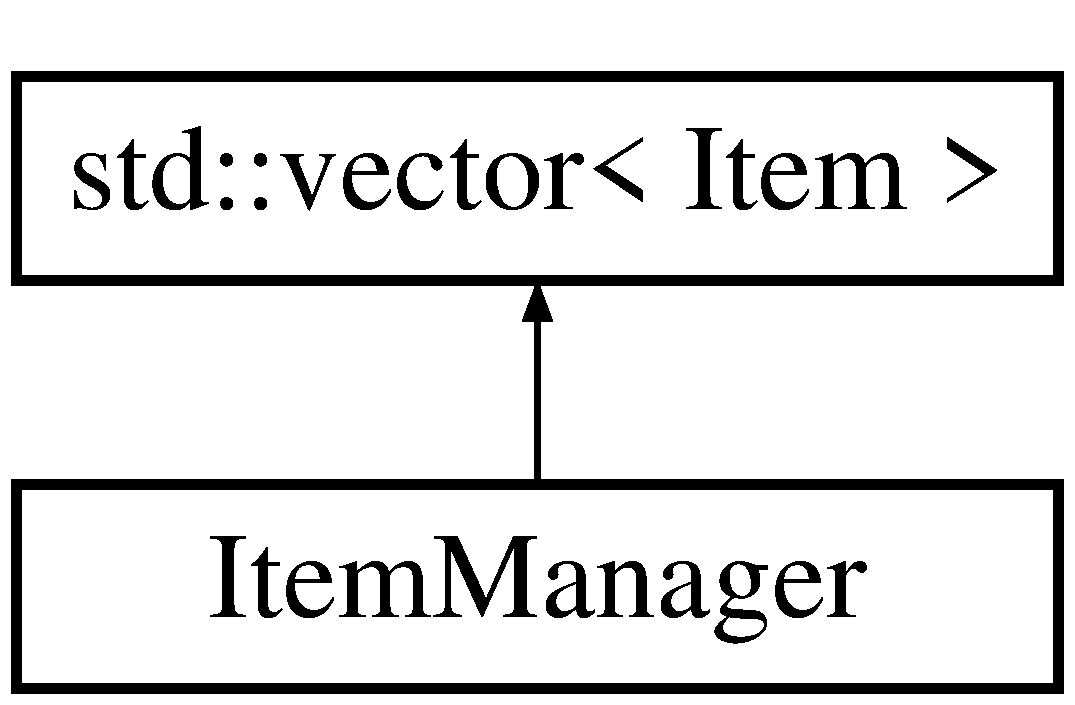
\includegraphics[height=2.000000cm]{class_item_manager}
\end{center}
\end{figure}
\subsection*{Public Member Functions}
\begin{DoxyCompactItemize}
\item 
void \mbox{\hyperlink{class_item_manager_ad3e190ba89c34cdaa4b11ecbdb6e8722}{display}} (std\+::ostream \&, bool=false) const
\end{DoxyCompactItemize}


\subsection{Member Function Documentation}
\mbox{\Hypertarget{class_item_manager_ad3e190ba89c34cdaa4b11ecbdb6e8722}\label{class_item_manager_ad3e190ba89c34cdaa4b11ecbdb6e8722}} 
\index{Item\+Manager@{Item\+Manager}!display@{display}}
\index{display@{display}!Item\+Manager@{Item\+Manager}}
\subsubsection{\texorpdfstring{display()}{display()}}
{\footnotesize\ttfamily void Item\+Manager\+::display (\begin{DoxyParamCaption}\item[{std\+::ostream \&}]{os,  }\item[{bool}]{full = {\ttfamily false} }\end{DoxyParamCaption}) const}

inserts into os descriptions of each item stored in the base class container. 
\begin{DoxyParams}{Parameters}
{\em full} & specifies whether a full description of the item should be inserted. \\
\hline
{\em os} & The os object to display to \\
\hline
\end{DoxyParams}


The documentation for this class was generated from the following files\+:\begin{DoxyCompactItemize}
\item 
\mbox{\hyperlink{_item_manager_8h}{Item\+Manager.\+h}}\item 
\mbox{\hyperlink{_item_manager_8cpp}{Item\+Manager.\+cpp}}\end{DoxyCompactItemize}

\hypertarget{class_order_manager}{}\section{Order\+Manager Class Reference}
\label{class_order_manager}\index{Order\+Manager@{Order\+Manager}}


{\ttfamily \#include $<$Order\+Manager.\+h$>$}

Inheritance diagram for Order\+Manager\+:\begin{figure}[H]
\begin{center}
\leavevmode
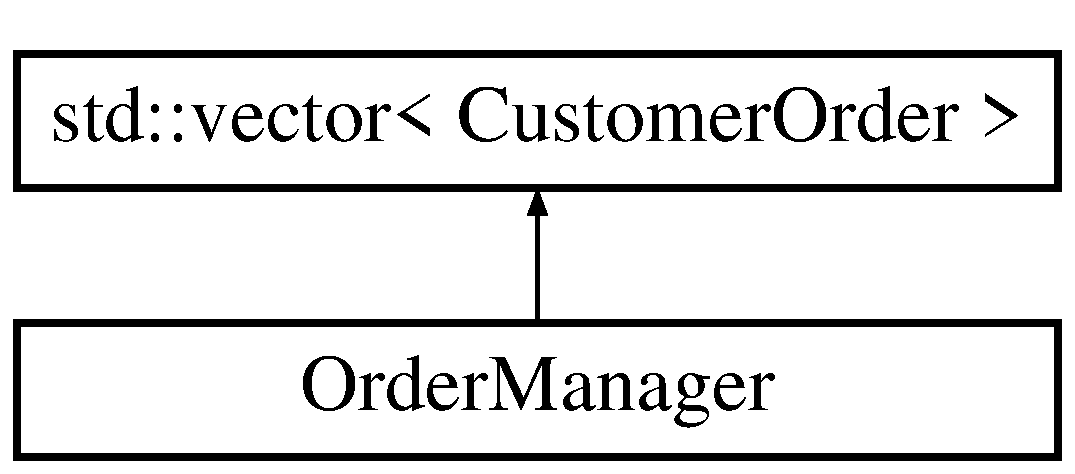
\includegraphics[height=2.000000cm]{class_order_manager}
\end{center}
\end{figure}
\subsection*{Public Member Functions}
\begin{DoxyCompactItemize}
\item 
\mbox{\hyperlink{class_customer_order}{Customer\+Order}} \&\& \mbox{\hyperlink{class_order_manager_a2111b67d23078421bb0c012c25ee87f1}{extract}} ()
\item 
void \mbox{\hyperlink{class_order_manager_a5469cae831246813134630f8bd85db79}{validate}} (const \mbox{\hyperlink{class_item_manager}{Item\+Manager}} \&, std\+::ostream \&)
\item 
void \mbox{\hyperlink{class_order_manager_a01ff4be0afbb0535de41d5caedcf0016}{display}} (std\+::ostream \&) const
\end{DoxyCompactItemize}


\subsection{Member Function Documentation}
\mbox{\Hypertarget{class_order_manager_a01ff4be0afbb0535de41d5caedcf0016}\label{class_order_manager_a01ff4be0afbb0535de41d5caedcf0016}} 
\index{Order\+Manager@{Order\+Manager}!display@{display}}
\index{display@{display}!Order\+Manager@{Order\+Manager}}
\subsubsection{\texorpdfstring{display()}{display()}}
{\footnotesize\ttfamily void Order\+Manager\+::display (\begin{DoxyParamCaption}\item[{std\+::ostream \&}]{os }\end{DoxyParamCaption}) const}

Displays the contents of Customer\+Orders in the vector \mbox{\Hypertarget{class_order_manager_a2111b67d23078421bb0c012c25ee87f1}\label{class_order_manager_a2111b67d23078421bb0c012c25ee87f1}} 
\index{Order\+Manager@{Order\+Manager}!extract@{extract}}
\index{extract@{extract}!Order\+Manager@{Order\+Manager}}
\subsubsection{\texorpdfstring{extract()}{extract()}}
{\footnotesize\ttfamily \mbox{\hyperlink{class_customer_order}{Customer\+Order}} \&\& Order\+Manager\+::extract (\begin{DoxyParamCaption}{ }\end{DoxyParamCaption})}

Extracts the last object from the vector \begin{DoxyReturn}{Returns}
A move reference to the last vector element 
\end{DoxyReturn}
\mbox{\Hypertarget{class_order_manager_a5469cae831246813134630f8bd85db79}\label{class_order_manager_a5469cae831246813134630f8bd85db79}} 
\index{Order\+Manager@{Order\+Manager}!validate@{validate}}
\index{validate@{validate}!Order\+Manager@{Order\+Manager}}
\subsubsection{\texorpdfstring{validate()}{validate()}}
{\footnotesize\ttfamily void Order\+Manager\+::validate (\begin{DoxyParamCaption}\item[{const \mbox{\hyperlink{class_item_manager}{Item\+Manager}} \&}]{im,  }\item[{std\+::ostream \&}]{os }\end{DoxyParamCaption})}

checks that the items requested in the customer orders are available. 
\begin{DoxyParams}{Parameters}
{\em im} & The item manager object with available items \\
\hline
{\em os} & The ostream object for error messages \\
\hline
\end{DoxyParams}


The documentation for this class was generated from the following files\+:\begin{DoxyCompactItemize}
\item 
\mbox{\hyperlink{_order_manager_8h}{Order\+Manager.\+h}}\item 
\mbox{\hyperlink{_order_manager_8cpp}{Order\+Manager.\+cpp}}\end{DoxyCompactItemize}

\hypertarget{class_task}{}\section{Task Class Reference}
\label{class_task}\index{Task@{Task}}


Holds the structure of a task.  




{\ttfamily \#include $<$Task.\+h$>$}

\subsection*{Public Types}
\begin{DoxyCompactItemize}
\item 
enum \mbox{\hyperlink{class_task_a6b8b1fc5858cbd77055e79d6381282fb}{Quality}} \{ \mbox{\hyperlink{class_task_a6b8b1fc5858cbd77055e79d6381282fbafc26836e15aeaddaab5eaca6d03dadba}{passed}}, 
\mbox{\hyperlink{class_task_a6b8b1fc5858cbd77055e79d6381282fba9a7ec146540b101a16e2da2bd61e5b59}{redirect}}
 \}
\begin{DoxyCompactList}\small\item\em Used to select the next task to complete. \end{DoxyCompactList}\end{DoxyCompactItemize}
\subsection*{Public Member Functions}
\begin{DoxyCompactItemize}
\item 
\mbox{\hyperlink{class_task_ace3ff25451f6d46f6cc0f2d7ed4b16ef}{Task}} (const std\+::string \&)
\begin{DoxyCompactList}\small\item\em Initalizes to a safe state, then reads the tokens from the parameter string to populate data. \end{DoxyCompactList}\item 
const std\+::string \& \mbox{\hyperlink{class_task_a0c1ae0dd618c9b8ae35591040d3776f3}{get\+Name}} () const
\begin{DoxyCompactList}\small\item\em Returns the name of the task. \end{DoxyCompactList}\item 
bool \mbox{\hyperlink{class_task_a974eb3143ac070fd67495f3c4a108a96}{validate}} (const \mbox{\hyperlink{class_task}{Task}} \&)
\begin{DoxyCompactList}\small\item\em Validates and stores the next tasks. \end{DoxyCompactList}\item 
unsigned int \mbox{\hyperlink{class_task_a67589413dbb0d5ffa3b2f08c6fa461ea}{get\+Slots}} () const
\begin{DoxyCompactList}\small\item\em Returns the number of production slots avaliable to the task. \end{DoxyCompactList}\item 
const \mbox{\hyperlink{class_task}{Task}} $\ast$ \mbox{\hyperlink{class_task_acf6851078d506896872fa7cc6476e5bf}{get\+Next\+Task}} (\mbox{\hyperlink{class_task_a6b8b1fc5858cbd77055e79d6381282fb}{Quality}}) const
\begin{DoxyCompactList}\small\item\em Returns the next task based on Quality. \end{DoxyCompactList}\item 
void \mbox{\hyperlink{class_task_aff00aecd7c14bd02434b76ad10a656a2}{display}} (std\+::ostream \&) const
\begin{DoxyCompactList}\small\item\em Displays the current task to the ostream object. \end{DoxyCompactList}\end{DoxyCompactItemize}
\subsection*{Static Public Member Functions}
\begin{DoxyCompactItemize}
\item 
static size\+\_\+t \mbox{\hyperlink{class_task_a18f265f8b4a37e5ed047034c2558068b}{get\+Field\+Width}} ()
\begin{DoxyCompactList}\small\item\em Returns the feild width for the class. \end{DoxyCompactList}\end{DoxyCompactItemize}


\subsection{Detailed Description}
Holds the structure of a task. 

\subsection{Member Enumeration Documentation}
\mbox{\Hypertarget{class_task_a6b8b1fc5858cbd77055e79d6381282fb}\label{class_task_a6b8b1fc5858cbd77055e79d6381282fb}} 
\index{Task@{Task}!Quality@{Quality}}
\index{Quality@{Quality}!Task@{Task}}
\subsubsection{\texorpdfstring{Quality}{Quality}}
{\footnotesize\ttfamily enum \mbox{\hyperlink{class_task_a6b8b1fc5858cbd77055e79d6381282fb}{Task\+::\+Quality}}}



Used to select the next task to complete. 

\begin{DoxyEnumFields}{Enumerator}
\raisebox{\heightof{T}}[0pt][0pt]{\index{passed@{passed}!Task@{Task}}\index{Task@{Task}!passed@{passed}}}\mbox{\Hypertarget{class_task_a6b8b1fc5858cbd77055e79d6381282fbafc26836e15aeaddaab5eaca6d03dadba}\label{class_task_a6b8b1fc5858cbd77055e79d6381282fbafc26836e15aeaddaab5eaca6d03dadba}} 
passed&\\
\hline

\raisebox{\heightof{T}}[0pt][0pt]{\index{redirect@{redirect}!Task@{Task}}\index{Task@{Task}!redirect@{redirect}}}\mbox{\Hypertarget{class_task_a6b8b1fc5858cbd77055e79d6381282fba9a7ec146540b101a16e2da2bd61e5b59}\label{class_task_a6b8b1fc5858cbd77055e79d6381282fba9a7ec146540b101a16e2da2bd61e5b59}} 
redirect&\\
\hline

\end{DoxyEnumFields}


\subsection{Constructor \& Destructor Documentation}
\mbox{\Hypertarget{class_task_ace3ff25451f6d46f6cc0f2d7ed4b16ef}\label{class_task_ace3ff25451f6d46f6cc0f2d7ed4b16ef}} 
\index{Task@{Task}!Task@{Task}}
\index{Task@{Task}!Task@{Task}}
\subsubsection{\texorpdfstring{Task()}{Task()}}
{\footnotesize\ttfamily Task\+::\+Task (\begin{DoxyParamCaption}\item[{const std\+::string \&}]{in }\end{DoxyParamCaption})}



Initalizes to a safe state, then reads the tokens from the parameter string to populate data. 

The constructor initializes the number of product slots to a default value of 1 and the pointers to the next tasks to safe addresses. The constructor then uses a \mbox{\hyperlink{class_utilities}{Utilities}} object to extract each token from the record. Once the constructor has extracted all of the tokens from the record, it retrieves the maximum field width needed by the extracted tokens. If that field width is greater than field\+\_\+width, the constructor resets this class variable to the value retrieved. 
\begin{DoxyParams}{Parameters}
{\em in} & -\/ a string which contains a single record in the structure of\+: Name $\vert$ Slots $\vert$ Success\+Task $\vert$ Fail\+Task \\
\hline
\end{DoxyParams}
\begin{DoxySeeAlso}{See also}
\mbox{\hyperlink{class_utilities_a59c27deae1e3810d8591b35ed90b7f33}{Utilities\+::next\+Token()}} 
\end{DoxySeeAlso}


\subsection{Member Function Documentation}
\mbox{\Hypertarget{class_task_aff00aecd7c14bd02434b76ad10a656a2}\label{class_task_aff00aecd7c14bd02434b76ad10a656a2}} 
\index{Task@{Task}!display@{display}}
\index{display@{display}!Task@{Task}}
\subsubsection{\texorpdfstring{display()}{display()}}
{\footnotesize\ttfamily void Task\+::display (\begin{DoxyParamCaption}\item[{std\+::ostream \&}]{os }\end{DoxyParamCaption}) const}



Displays the current task to the ostream object. 

uses the field width to display the name, slots and next task(s) in the current object. Throws exception if string is empty. 
\begin{DoxyParams}{Parameters}
{\em os} & The ostream object to output to \\
\hline
\end{DoxyParams}
\mbox{\Hypertarget{class_task_a18f265f8b4a37e5ed047034c2558068b}\label{class_task_a18f265f8b4a37e5ed047034c2558068b}} 
\index{Task@{Task}!get\+Field\+Width@{get\+Field\+Width}}
\index{get\+Field\+Width@{get\+Field\+Width}!Task@{Task}}
\subsubsection{\texorpdfstring{get\+Field\+Width()}{getFieldWidth()}}
{\footnotesize\ttfamily static size\+\_\+t Task\+::get\+Field\+Width (\begin{DoxyParamCaption}{ }\end{DoxyParamCaption})\hspace{0.3cm}{\ttfamily [inline]}, {\ttfamily [static]}}



Returns the feild width for the class. 

\begin{DoxyReturn}{Returns}
size\+\_\+t of the feild width from the tokens that have been stored in the class 
\end{DoxyReturn}
\mbox{\Hypertarget{class_task_a0c1ae0dd618c9b8ae35591040d3776f3}\label{class_task_a0c1ae0dd618c9b8ae35591040d3776f3}} 
\index{Task@{Task}!get\+Name@{get\+Name}}
\index{get\+Name@{get\+Name}!Task@{Task}}
\subsubsection{\texorpdfstring{get\+Name()}{getName()}}
{\footnotesize\ttfamily const std\+::string \& Task\+::get\+Name (\begin{DoxyParamCaption}{ }\end{DoxyParamCaption}) const}



Returns the name of the task. 

\begin{DoxyReturn}{Returns}
Const reference to the task name. 
\end{DoxyReturn}
\mbox{\Hypertarget{class_task_acf6851078d506896872fa7cc6476e5bf}\label{class_task_acf6851078d506896872fa7cc6476e5bf}} 
\index{Task@{Task}!get\+Next\+Task@{get\+Next\+Task}}
\index{get\+Next\+Task@{get\+Next\+Task}!Task@{Task}}
\subsubsection{\texorpdfstring{get\+Next\+Task()}{getNextTask()}}
{\footnotesize\ttfamily const \mbox{\hyperlink{class_task}{Task}} $\ast$ Task\+::get\+Next\+Task (\begin{DoxyParamCaption}\item[{\mbox{\hyperlink{class_task_a6b8b1fc5858cbd77055e79d6381282fb}{Quality}}}]{q }\end{DoxyParamCaption}) const}



Returns the next task based on Quality. 

The selected Quality is used to select which of the stored tasks should be next. 
\begin{DoxyParams}{Parameters}
{\em q} & -\/ The Quality that has been selected \\
\hline
\end{DoxyParams}
\begin{DoxyReturn}{Returns}
A reference to the selected task 
\end{DoxyReturn}
\begin{DoxySeeAlso}{See also}
\mbox{\hyperlink{class_task_a6b8b1fc5858cbd77055e79d6381282fb}{Quality}} 
\end{DoxySeeAlso}
\mbox{\Hypertarget{class_task_a67589413dbb0d5ffa3b2f08c6fa461ea}\label{class_task_a67589413dbb0d5ffa3b2f08c6fa461ea}} 
\index{Task@{Task}!get\+Slots@{get\+Slots}}
\index{get\+Slots@{get\+Slots}!Task@{Task}}
\subsubsection{\texorpdfstring{get\+Slots()}{getSlots()}}
{\footnotesize\ttfamily unsigned int Task\+::get\+Slots (\begin{DoxyParamCaption}{ }\end{DoxyParamCaption}) const}



Returns the number of production slots avaliable to the task. 

\begin{DoxyReturn}{Returns}
An integer of the slots converted from string 
\end{DoxyReturn}
\mbox{\Hypertarget{class_task_a974eb3143ac070fd67495f3c4a108a96}\label{class_task_a974eb3143ac070fd67495f3c4a108a96}} 
\index{Task@{Task}!validate@{validate}}
\index{validate@{validate}!Task@{Task}}
\subsubsection{\texorpdfstring{validate()}{validate()}}
{\footnotesize\ttfamily bool Task\+::validate (\begin{DoxyParamCaption}\item[{const \mbox{\hyperlink{class_task}{Task}} \&}]{task }\end{DoxyParamCaption})}



Validates and stores the next tasks. 

compares the name of the parameter task to the next tasks stored in the current object. If the names match the address of the passed task is stored. 
\begin{DoxyParams}{Parameters}
{\em task} & -\/ Reference to the task to validate against \\
\hline
\end{DoxyParams}
\begin{DoxyReturn}{Returns}
Boolean -\/ true if both tasks in the object either point to another task object, or have no name. 
\end{DoxyReturn}


The documentation for this class was generated from the following files\+:\begin{DoxyCompactItemize}
\item 
\mbox{\hyperlink{_task_8h}{Task.\+h}}\item 
\mbox{\hyperlink{_task_8cpp}{Task.\+cpp}}\end{DoxyCompactItemize}

\hypertarget{class_task_manager}{}\section{Task\+Manager Class Reference}
\label{class_task_manager}\index{Task\+Manager@{Task\+Manager}}


{\ttfamily \#include $<$Task\+Manager.\+h$>$}

Inheritance diagram for Task\+Manager\+:\begin{figure}[H]
\begin{center}
\leavevmode
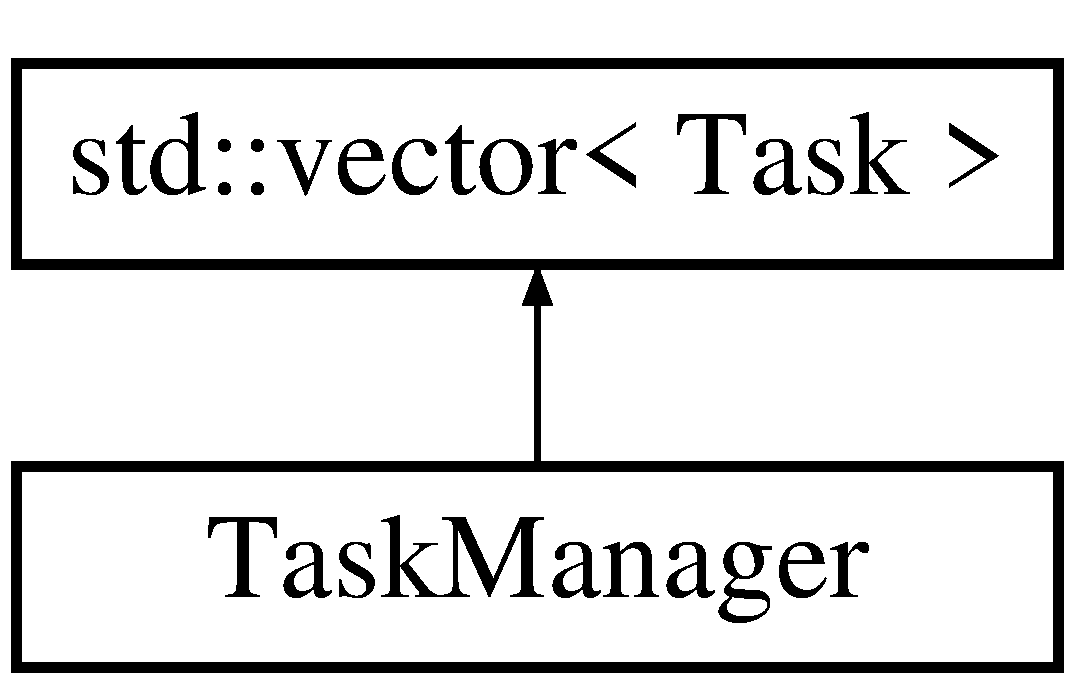
\includegraphics[height=2.000000cm]{class_task_manager}
\end{center}
\end{figure}
\subsection*{Public Member Functions}
\begin{DoxyCompactItemize}
\item 
void \mbox{\hyperlink{class_task_manager_a2ae3c30ca4e030440b64c383cbda8a73}{validate}} (std\+::ostream \&)
\item 
void \mbox{\hyperlink{class_task_manager_a59aea57b2ad273d6d95797f93d737fa0}{validate}} (const \mbox{\hyperlink{class_item_manager}{Item\+Manager}} \&, std\+::ostream \&)
\item 
void \mbox{\hyperlink{class_task_manager_a3564901af8fa7498b0fcca85fcaa5e64}{display}} (std\+::ostream \&) const
\end{DoxyCompactItemize}


\subsection{Member Function Documentation}
\mbox{\Hypertarget{class_task_manager_a3564901af8fa7498b0fcca85fcaa5e64}\label{class_task_manager_a3564901af8fa7498b0fcca85fcaa5e64}} 
\index{Task\+Manager@{Task\+Manager}!display@{display}}
\index{display@{display}!Task\+Manager@{Task\+Manager}}
\subsubsection{\texorpdfstring{display()}{display()}}
{\footnotesize\ttfamily void Task\+Manager\+::display (\begin{DoxyParamCaption}\item[{std\+::ostream \&}]{os }\end{DoxyParamCaption}) const}

Displays the contents of Tasks in the vector \mbox{\Hypertarget{class_task_manager_a2ae3c30ca4e030440b64c383cbda8a73}\label{class_task_manager_a2ae3c30ca4e030440b64c383cbda8a73}} 
\index{Task\+Manager@{Task\+Manager}!validate@{validate}}
\index{validate@{validate}!Task\+Manager@{Task\+Manager}}
\subsubsection{\texorpdfstring{validate()}{validate()}\hspace{0.1cm}{\footnotesize\ttfamily [1/2]}}
{\footnotesize\ttfamily void Task\+Manager\+::validate (\begin{DoxyParamCaption}\item[{std\+::ostream \&}]{os }\end{DoxyParamCaption})}

Validates all Tasks in the vector 
\begin{DoxyParams}{Parameters}
{\em os} & Error Message output \\
\hline
\end{DoxyParams}
\mbox{\Hypertarget{class_task_manager_a59aea57b2ad273d6d95797f93d737fa0}\label{class_task_manager_a59aea57b2ad273d6d95797f93d737fa0}} 
\index{Task\+Manager@{Task\+Manager}!validate@{validate}}
\index{validate@{validate}!Task\+Manager@{Task\+Manager}}
\subsubsection{\texorpdfstring{validate()}{validate()}\hspace{0.1cm}{\footnotesize\ttfamily [2/2]}}
{\footnotesize\ttfamily void Task\+Manager\+::validate (\begin{DoxyParamCaption}\item[{const \mbox{\hyperlink{class_item_manager}{Item\+Manager}} \&}]{im,  }\item[{std\+::ostream \&}]{os }\end{DoxyParamCaption})}

Validates all Tasks used by items in \mbox{\hyperlink{class_item}{Item}} Manager are in the vector 
\begin{DoxyParams}{Parameters}
{\em im} & The \mbox{\hyperlink{class_item}{Item}} Manager \\
\hline
{\em os} & Error Message output \\
\hline
\end{DoxyParams}


The documentation for this class was generated from the following files\+:\begin{DoxyCompactItemize}
\item 
\mbox{\hyperlink{_task_manager_8h}{Task\+Manager.\+h}}\item 
\mbox{\hyperlink{_task_manager_8cpp}{Task\+Manager.\+cpp}}\end{DoxyCompactItemize}

\hypertarget{class_utilities}{}\section{Utilities Class Reference}
\label{class_utilities}\index{Utilities@{Utilities}}


Holds various utilities.  




{\ttfamily \#include $<$Utilities.\+h$>$}

\subsection*{Public Member Functions}
\begin{DoxyCompactItemize}
\item 
\mbox{\hyperlink{class_utilities_ab1676c9ce35cf347a73d16f1094e1271}{Utilities}} ()
\begin{DoxyCompactList}\small\item\em Sets field width to 1. \end{DoxyCompactList}\item 
void \mbox{\hyperlink{class_utilities_a90cee9218e3faff9bd060beda0e83e17}{set\+Field\+Width}} (size\+\_\+t fw)
\begin{DoxyCompactList}\small\item\em Sets the objects field width. \end{DoxyCompactList}\item 
size\+\_\+t \mbox{\hyperlink{class_utilities_a94abc3ceade71097979e76e15008efba}{get\+Field\+Width}} () const
\begin{DoxyCompactList}\small\item\em Gets the objects field width. \end{DoxyCompactList}\item 
const std\+::string \mbox{\hyperlink{class_utilities_a59c27deae1e3810d8591b35ed90b7f33}{next\+Token}} (const std\+::string \&, size\+\_\+t \&, bool \&)
\begin{DoxyCompactList}\small\item\em gets the next token in a string \end{DoxyCompactList}\item 
int \mbox{\hyperlink{class_utilities_a8f3e9e16a823944a3bdb67c6c3d70d08}{ftrim}} (std\+::string \&str)
\begin{DoxyCompactList}\small\item\em trims whitespace from the front of a string \end{DoxyCompactList}\item 
int \mbox{\hyperlink{class_utilities_afffccc73f8e56740fdf789904bf268ee}{rtrim}} (std\+::string \&str)
\begin{DoxyCompactList}\small\item\em trims whitespace from the back of a string \end{DoxyCompactList}\item 
int \mbox{\hyperlink{class_utilities_ac71774c0324d441f542665f8f372a113}{trim}} (std\+::string \&str)
\begin{DoxyCompactList}\small\item\em trims whitespace from a string \end{DoxyCompactList}\end{DoxyCompactItemize}
\subsection*{Static Public Member Functions}
\begin{DoxyCompactItemize}
\item 
static void \mbox{\hyperlink{class_utilities_a5d0e249841a1ec89395a1810fa81354f}{set\+Delimiter}} (const char del)
\begin{DoxyCompactList}\small\item\em sets the class variable delimiter \end{DoxyCompactList}\item 
static void \mbox{\hyperlink{class_utilities_a4d03fd38f07e567277b82b8a0e030245}{set\+Log\+File}} (const char $\ast$log)
\begin{DoxyCompactList}\small\item\em Opens a log file held in the class variable log\+File. \end{DoxyCompactList}\item 
static std\+::ofstream \& \mbox{\hyperlink{class_utilities_aecd7de50b27a709a9810b17940074cad}{get\+Log\+File}} ()
\begin{DoxyCompactList}\small\item\em Gets the log\+File reference. \end{DoxyCompactList}\end{DoxyCompactItemize}


\subsection{Detailed Description}
Holds various utilities. 

\subsection{Constructor \& Destructor Documentation}
\mbox{\Hypertarget{class_utilities_ab1676c9ce35cf347a73d16f1094e1271}\label{class_utilities_ab1676c9ce35cf347a73d16f1094e1271}} 
\index{Utilities@{Utilities}!Utilities@{Utilities}}
\index{Utilities@{Utilities}!Utilities@{Utilities}}
\subsubsection{\texorpdfstring{Utilities()}{Utilities()}}
{\footnotesize\ttfamily Utilities\+::\+Utilities (\begin{DoxyParamCaption}{ }\end{DoxyParamCaption})}



Sets field width to 1. 



\subsection{Member Function Documentation}
\mbox{\Hypertarget{class_utilities_a8f3e9e16a823944a3bdb67c6c3d70d08}\label{class_utilities_a8f3e9e16a823944a3bdb67c6c3d70d08}} 
\index{Utilities@{Utilities}!ftrim@{ftrim}}
\index{ftrim@{ftrim}!Utilities@{Utilities}}
\subsubsection{\texorpdfstring{ftrim()}{ftrim()}}
{\footnotesize\ttfamily int Utilities\+::ftrim (\begin{DoxyParamCaption}\item[{std\+::string \&}]{str }\end{DoxyParamCaption})}



trims whitespace from the front of a string 


\begin{DoxyParams}{Parameters}
{\em str} & the string to trim \\
\hline
\end{DoxyParams}
\begin{DoxyReturn}{Returns}
the number of characters trimmed 
\end{DoxyReturn}
\mbox{\Hypertarget{class_utilities_a94abc3ceade71097979e76e15008efba}\label{class_utilities_a94abc3ceade71097979e76e15008efba}} 
\index{Utilities@{Utilities}!get\+Field\+Width@{get\+Field\+Width}}
\index{get\+Field\+Width@{get\+Field\+Width}!Utilities@{Utilities}}
\subsubsection{\texorpdfstring{get\+Field\+Width()}{getFieldWidth()}}
{\footnotesize\ttfamily size\+\_\+t Utilities\+::get\+Field\+Width (\begin{DoxyParamCaption}{ }\end{DoxyParamCaption}) const}



Gets the objects field width. 

\mbox{\Hypertarget{class_utilities_aecd7de50b27a709a9810b17940074cad}\label{class_utilities_aecd7de50b27a709a9810b17940074cad}} 
\index{Utilities@{Utilities}!get\+Log\+File@{get\+Log\+File}}
\index{get\+Log\+File@{get\+Log\+File}!Utilities@{Utilities}}
\subsubsection{\texorpdfstring{get\+Log\+File()}{getLogFile()}}
{\footnotesize\ttfamily static std\+::ofstream\& Utilities\+::get\+Log\+File (\begin{DoxyParamCaption}{ }\end{DoxyParamCaption})\hspace{0.3cm}{\ttfamily [inline]}, {\ttfamily [static]}}



Gets the log\+File reference. 

\begin{DoxyReturn}{Returns}
A reference to the ofstream class variable log\+File 
\end{DoxyReturn}
\begin{DoxySeeAlso}{See also}
\mbox{\hyperlink{class_utilities_a4d03fd38f07e567277b82b8a0e030245}{set\+Log\+File()}} 
\end{DoxySeeAlso}
\mbox{\Hypertarget{class_utilities_a59c27deae1e3810d8591b35ed90b7f33}\label{class_utilities_a59c27deae1e3810d8591b35ed90b7f33}} 
\index{Utilities@{Utilities}!next\+Token@{next\+Token}}
\index{next\+Token@{next\+Token}!Utilities@{Utilities}}
\subsubsection{\texorpdfstring{next\+Token()}{nextToken()}}
{\footnotesize\ttfamily const std\+::string Utilities\+::next\+Token (\begin{DoxyParamCaption}\item[{const std\+::string \&}]{in,  }\item[{size\+\_\+t \&}]{pos,  }\item[{bool \&}]{more }\end{DoxyParamCaption})}



gets the next token in a string 

Reads from the provided position in the string until the delimeter in the object is found. Returns a trimmed string from pos to the next delimeter. Sets the feild width to that length if the current field width is shorter. Adds string length, trimmed characters, and 1 to remove delim to pos. Throws exception if string is empty. 
\begin{DoxyParams}{Parameters}
{\em in} & The input string \\
\hline
{\em pos} & The position to start reading from, returns the position that it stopped reading. \\
\hline
{\em more} & Changes the more boolean to true if there is more to read after the delimeter. \\
\hline
\end{DoxyParams}
\begin{DoxyReturn}{Returns}
trimmed string from pos to the next delimeter 
\end{DoxyReturn}
\begin{DoxySeeAlso}{See also}
\mbox{\hyperlink{class_utilities_ac71774c0324d441f542665f8f372a113}{trim()}}, \mbox{\hyperlink{class_utilities_a5d0e249841a1ec89395a1810fa81354f}{set\+Delimiter()}} and \mbox{\hyperlink{class_utilities_a90cee9218e3faff9bd060beda0e83e17}{set\+Field\+Width()}} 
\end{DoxySeeAlso}
\mbox{\Hypertarget{class_utilities_afffccc73f8e56740fdf789904bf268ee}\label{class_utilities_afffccc73f8e56740fdf789904bf268ee}} 
\index{Utilities@{Utilities}!rtrim@{rtrim}}
\index{rtrim@{rtrim}!Utilities@{Utilities}}
\subsubsection{\texorpdfstring{rtrim()}{rtrim()}}
{\footnotesize\ttfamily int Utilities\+::rtrim (\begin{DoxyParamCaption}\item[{std\+::string \&}]{str }\end{DoxyParamCaption})}



trims whitespace from the back of a string 


\begin{DoxyParams}{Parameters}
{\em str} & the string to trim \\
\hline
\end{DoxyParams}
\begin{DoxyReturn}{Returns}
the number of characters trimmed 
\end{DoxyReturn}
\mbox{\Hypertarget{class_utilities_a5d0e249841a1ec89395a1810fa81354f}\label{class_utilities_a5d0e249841a1ec89395a1810fa81354f}} 
\index{Utilities@{Utilities}!set\+Delimiter@{set\+Delimiter}}
\index{set\+Delimiter@{set\+Delimiter}!Utilities@{Utilities}}
\subsubsection{\texorpdfstring{set\+Delimiter()}{setDelimiter()}}
{\footnotesize\ttfamily static void Utilities\+::set\+Delimiter (\begin{DoxyParamCaption}\item[{const char}]{del }\end{DoxyParamCaption})\hspace{0.3cm}{\ttfamily [inline]}, {\ttfamily [static]}}



sets the class variable delimiter 


\begin{DoxyParams}{Parameters}
{\em del} & char to set the delimiter to. \\
\hline
\end{DoxyParams}
\mbox{\Hypertarget{class_utilities_a90cee9218e3faff9bd060beda0e83e17}\label{class_utilities_a90cee9218e3faff9bd060beda0e83e17}} 
\index{Utilities@{Utilities}!set\+Field\+Width@{set\+Field\+Width}}
\index{set\+Field\+Width@{set\+Field\+Width}!Utilities@{Utilities}}
\subsubsection{\texorpdfstring{set\+Field\+Width()}{setFieldWidth()}}
{\footnotesize\ttfamily void Utilities\+::set\+Field\+Width (\begin{DoxyParamCaption}\item[{size\+\_\+t}]{fw }\end{DoxyParamCaption})}



Sets the objects field width. 


\begin{DoxyParams}{Parameters}
{\em fw} & -\/ the value for the feild width of the object \\
\hline
\end{DoxyParams}
\begin{DoxySeeAlso}{See also}
get\+Feild\+Width() 
\end{DoxySeeAlso}
\mbox{\Hypertarget{class_utilities_a4d03fd38f07e567277b82b8a0e030245}\label{class_utilities_a4d03fd38f07e567277b82b8a0e030245}} 
\index{Utilities@{Utilities}!set\+Log\+File@{set\+Log\+File}}
\index{set\+Log\+File@{set\+Log\+File}!Utilities@{Utilities}}
\subsubsection{\texorpdfstring{set\+Log\+File()}{setLogFile()}}
{\footnotesize\ttfamily static void Utilities\+::set\+Log\+File (\begin{DoxyParamCaption}\item[{const char $\ast$}]{log }\end{DoxyParamCaption})\hspace{0.3cm}{\ttfamily [inline]}, {\ttfamily [static]}}



Opens a log file held in the class variable log\+File. 


\begin{DoxyParams}{Parameters}
{\em log} & filename to open in trunc mode \\
\hline
\end{DoxyParams}
\mbox{\Hypertarget{class_utilities_ac71774c0324d441f542665f8f372a113}\label{class_utilities_ac71774c0324d441f542665f8f372a113}} 
\index{Utilities@{Utilities}!trim@{trim}}
\index{trim@{trim}!Utilities@{Utilities}}
\subsubsection{\texorpdfstring{trim()}{trim()}}
{\footnotesize\ttfamily int Utilities\+::trim (\begin{DoxyParamCaption}\item[{std\+::string \&}]{str }\end{DoxyParamCaption})}



trims whitespace from a string 


\begin{DoxyParams}{Parameters}
{\em str} & the string to trim \\
\hline
\end{DoxyParams}
\begin{DoxyReturn}{Returns}
the number of characters trimmed 
\end{DoxyReturn}
\begin{DoxySeeAlso}{See also}
\mbox{\hyperlink{class_utilities_a8f3e9e16a823944a3bdb67c6c3d70d08}{ftrim()}} and \mbox{\hyperlink{class_utilities_afffccc73f8e56740fdf789904bf268ee}{rtrim()}} 
\end{DoxySeeAlso}


The documentation for this class was generated from the following files\+:\begin{DoxyCompactItemize}
\item 
\mbox{\hyperlink{_utilities_8h}{Utilities.\+h}}\item 
\mbox{\hyperlink{_utilities_8cpp}{Utilities.\+cpp}}\end{DoxyCompactItemize}

\chapter{File Documentation}
\hypertarget{_8cpp}{}\section{.cpp File Reference}
\label{_8cpp}\index{.\+cpp@{.\+cpp}}
{\ttfamily \#include $<$iostream$>$}\newline
{\ttfamily \#include $<$fstream$>$}\newline
{\ttfamily \#include $<$string$>$}\newline
{\ttfamily \#include $<$cstdlib$>$}\newline
{\ttfamily \#include $<$vector$>$}\newline
{\ttfamily \#include $<$memory$>$}\newline
{\ttfamily \#include \char`\"{}Customer\+Order.\+h\char`\"{}}\newline
{\ttfamily \#include \char`\"{}Utilities.\+h\char`\"{}}\newline
{\ttfamily \#include \char`\"{}Item.\+h\char`\"{}}\newline
\subsection*{Functions}
\begin{DoxyCompactItemize}
\item 
{\footnotesize template$<$typename T $>$ }\\void \mbox{\hyperlink{_8cpp_a720822ee36812c01e9e2559d17233647}{load\+From\+File}} (const char $\ast$, std\+::vector$<$ T $>$ \&, std\+::ostream \&)
\item 
int \mbox{\hyperlink{_8cpp_a3c04138a5bfe5d72780bb7e82a18e627}{main}} (int argc, char $\ast$$\ast$argv)
\end{DoxyCompactItemize}


\subsection{Function Documentation}
\mbox{\Hypertarget{_8cpp_a720822ee36812c01e9e2559d17233647}\label{_8cpp_a720822ee36812c01e9e2559d17233647}} 
\index{.\+cpp@{.\+cpp}!load\+From\+File@{load\+From\+File}}
\index{load\+From\+File@{load\+From\+File}!.\+cpp@{.\+cpp}}
\subsubsection{\texorpdfstring{load\+From\+File()}{loadFromFile()}}
{\footnotesize\ttfamily template$<$typename T $>$ \\
void load\+From\+File (\begin{DoxyParamCaption}\item[{const char $\ast$}]{file\+Name,  }\item[{std\+::vector$<$ T $>$ \&}]{collection,  }\item[{std\+::ostream \&}]{os }\end{DoxyParamCaption})}

\mbox{\Hypertarget{_8cpp_a3c04138a5bfe5d72780bb7e82a18e627}\label{_8cpp_a3c04138a5bfe5d72780bb7e82a18e627}} 
\index{.\+cpp@{.\+cpp}!main@{main}}
\index{main@{main}!.\+cpp@{.\+cpp}}
\subsubsection{\texorpdfstring{main()}{main()}}
{\footnotesize\ttfamily int main (\begin{DoxyParamCaption}\item[{int}]{argc,  }\item[{char $\ast$$\ast$}]{argv }\end{DoxyParamCaption})}


\hypertarget{_customer_item_8cpp}{}\section{Customer\+Item.\+cpp File Reference}
\label{_customer_item_8cpp}\index{Customer\+Item.\+cpp@{Customer\+Item.\+cpp}}
{\ttfamily \#include \char`\"{}Customer\+Item.\+h\char`\"{}}\newline

\hypertarget{_customer_item_8h}{}\section{Customer\+Item.\+h File Reference}
\label{_customer_item_8h}\index{Customer\+Item.\+h@{Customer\+Item.\+h}}
{\ttfamily \#include $<$iostream$>$}\newline
{\ttfamily \#include $<$string$>$}\newline
{\ttfamily \#include \char`\"{}Item.\+h\char`\"{}}\newline
\subsection*{Classes}
\begin{DoxyCompactItemize}
\item 
class \mbox{\hyperlink{class_customer_item}{Customer\+Item}}
\end{DoxyCompactItemize}

\hypertarget{_customer_order_8cpp}{}\section{Customer\+Order.\+cpp File Reference}
\label{_customer_order_8cpp}\index{Customer\+Order.\+cpp@{Customer\+Order.\+cpp}}
{\ttfamily \#include \char`\"{}Customer\+Order.\+h\char`\"{}}\newline

\hypertarget{_customer_order_8h}{}\section{Customer\+Order.\+h File Reference}
\label{_customer_order_8h}\index{Customer\+Order.\+h@{Customer\+Order.\+h}}
{\ttfamily \#include $<$iostream$>$}\newline
{\ttfamily \#include $<$string$>$}\newline
{\ttfamily \#include \char`\"{}Utilities.\+h\char`\"{}}\newline
{\ttfamily \#include \char`\"{}Item.\+h\char`\"{}}\newline
{\ttfamily \#include \char`\"{}Customer\+Item.\+h\char`\"{}}\newline
\subsection*{Classes}
\begin{DoxyCompactItemize}
\item 
class \mbox{\hyperlink{class_customer_order}{Customer\+Order}}
\end{DoxyCompactItemize}
\subsection*{Macros}
\begin{DoxyCompactItemize}
\item 
\#define \mbox{\hyperlink{_customer_order_8h_a10a59554805ac7ce3905fd3540f98137}{N\+O\+E\+X\+C\+E\+PT}}
\end{DoxyCompactItemize}


\subsection{Macro Definition Documentation}
\mbox{\Hypertarget{_customer_order_8h_a10a59554805ac7ce3905fd3540f98137}\label{_customer_order_8h_a10a59554805ac7ce3905fd3540f98137}} 
\index{Customer\+Order.\+h@{Customer\+Order.\+h}!N\+O\+E\+X\+C\+E\+PT@{N\+O\+E\+X\+C\+E\+PT}}
\index{N\+O\+E\+X\+C\+E\+PT@{N\+O\+E\+X\+C\+E\+PT}!Customer\+Order.\+h@{Customer\+Order.\+h}}
\subsubsection{\texorpdfstring{N\+O\+E\+X\+C\+E\+PT}{NOEXCEPT}}
{\footnotesize\ttfamily \#define N\+O\+E\+X\+C\+E\+PT}


\hypertarget{_item_8cpp}{}\section{Item.\+cpp File Reference}
\label{_item_8cpp}\index{Item.\+cpp@{Item.\+cpp}}
{\ttfamily \#include \char`\"{}Item.\+h\char`\"{}}\newline

\hypertarget{_item_8h}{}\section{Item.\+h File Reference}
\label{_item_8h}\index{Item.\+h@{Item.\+h}}
{\ttfamily \#include $<$iostream$>$}\newline
{\ttfamily \#include $<$string$>$}\newline
{\ttfamily \#include \char`\"{}Utilities.\+h\char`\"{}}\newline
\subsection*{Classes}
\begin{DoxyCompactItemize}
\item 
class \mbox{\hyperlink{class_item}{Item}}
\end{DoxyCompactItemize}
\subsection*{Variables}
\begin{DoxyCompactItemize}
\item 
const unsigned int \mbox{\hyperlink{_item_8h_ae923513243df5de84b0dc0b0beb8a953}{C\+O\+D\+E\+\_\+\+W\+I\+D\+TH}} = 5
\end{DoxyCompactItemize}


\subsection{Variable Documentation}
\mbox{\Hypertarget{_item_8h_ae923513243df5de84b0dc0b0beb8a953}\label{_item_8h_ae923513243df5de84b0dc0b0beb8a953}} 
\index{Item.\+h@{Item.\+h}!C\+O\+D\+E\+\_\+\+W\+I\+D\+TH@{C\+O\+D\+E\+\_\+\+W\+I\+D\+TH}}
\index{C\+O\+D\+E\+\_\+\+W\+I\+D\+TH@{C\+O\+D\+E\+\_\+\+W\+I\+D\+TH}!Item.\+h@{Item.\+h}}
\subsubsection{\texorpdfstring{C\+O\+D\+E\+\_\+\+W\+I\+D\+TH}{CODE\_WIDTH}}
{\footnotesize\ttfamily const unsigned int C\+O\+D\+E\+\_\+\+W\+I\+D\+TH = 5}


\hypertarget{_item_manager_8cpp}{}\section{Item\+Manager.\+cpp File Reference}
\label{_item_manager_8cpp}\index{Item\+Manager.\+cpp@{Item\+Manager.\+cpp}}
{\ttfamily \#include \char`\"{}Item\+Manager.\+h\char`\"{}}\newline
{\ttfamily \#include $<$algorithm$>$}\newline

\hypertarget{_item_manager_8h}{}\section{Item\+Manager.\+h File Reference}
\label{_item_manager_8h}\index{Item\+Manager.\+h@{Item\+Manager.\+h}}
{\ttfamily \#include $<$iostream$>$}\newline
{\ttfamily \#include $<$vector$>$}\newline
{\ttfamily \#include \char`\"{}Item.\+h\char`\"{}}\newline
\subsection*{Classes}
\begin{DoxyCompactItemize}
\item 
class \mbox{\hyperlink{class_item_manager}{Item\+Manager}}
\end{DoxyCompactItemize}

\hypertarget{_milestone__3_8cpp}{}\section{Milestone\+\_\+3.\+cpp File Reference}
\label{_milestone__3_8cpp}\index{Milestone\+\_\+3.\+cpp@{Milestone\+\_\+3.\+cpp}}
{\ttfamily \#include $<$iostream$>$}\newline
{\ttfamily \#include $<$fstream$>$}\newline
{\ttfamily \#include $<$string$>$}\newline
{\ttfamily \#include $<$memory$>$}\newline
{\ttfamily \#include \char`\"{}Task.\+h\char`\"{}}\newline
{\ttfamily \#include \char`\"{}Task\+Manager.\+h\char`\"{}}\newline
{\ttfamily \#include \char`\"{}Customer\+Order.\+h\char`\"{}}\newline
{\ttfamily \#include \char`\"{}Order\+Manager.\+h\char`\"{}}\newline
{\ttfamily \#include \char`\"{}Item.\+h\char`\"{}}\newline
{\ttfamily \#include \char`\"{}Item\+Manager.\+h\char`\"{}}\newline
{\ttfamily \#include \char`\"{}Utilities.\+h\char`\"{}}\newline
\subsection*{Functions}
\begin{DoxyCompactItemize}
\item 
{\footnotesize template$<$typename M , typename T $>$ }\\void \mbox{\hyperlink{_milestone__3_8cpp_a5ed32e053f07a9a4297108f9cebc2c46}{load\+From\+File}} (const char $\ast$, M \&, std\+::ostream \&)
\item 
{\footnotesize template$<$$>$ }\\void \mbox{\hyperlink{_milestone__3_8cpp_accc12cc30ab8bcc74ba12ebd63858151}{load\+From\+File$<$ Task\+Manager, Task $>$}} (const char $\ast$, \mbox{\hyperlink{class_task_manager}{Task\+Manager}} \&, std\+::ostream \&)
\item 
int \mbox{\hyperlink{_milestone__3_8cpp_a3c04138a5bfe5d72780bb7e82a18e627}{main}} (int argc, char $\ast$$\ast$argv)
\end{DoxyCompactItemize}


\subsection{Function Documentation}
\mbox{\Hypertarget{_milestone__3_8cpp_a5ed32e053f07a9a4297108f9cebc2c46}\label{_milestone__3_8cpp_a5ed32e053f07a9a4297108f9cebc2c46}} 
\index{Milestone\+\_\+3.\+cpp@{Milestone\+\_\+3.\+cpp}!load\+From\+File@{load\+From\+File}}
\index{load\+From\+File@{load\+From\+File}!Milestone\+\_\+3.\+cpp@{Milestone\+\_\+3.\+cpp}}
\subsubsection{\texorpdfstring{load\+From\+File()}{loadFromFile()}}
{\footnotesize\ttfamily template$<$typename M , typename T $>$ \\
void load\+From\+File (\begin{DoxyParamCaption}\item[{const char $\ast$}]{file\+Name,  }\item[{M \&}]{manager,  }\item[{std\+::ostream \&}]{os }\end{DoxyParamCaption})}

\mbox{\Hypertarget{_milestone__3_8cpp_accc12cc30ab8bcc74ba12ebd63858151}\label{_milestone__3_8cpp_accc12cc30ab8bcc74ba12ebd63858151}} 
\index{Milestone\+\_\+3.\+cpp@{Milestone\+\_\+3.\+cpp}!load\+From\+File$<$ Task\+Manager, Task $>$@{load\+From\+File$<$ Task\+Manager, Task $>$}}
\index{load\+From\+File$<$ Task\+Manager, Task $>$@{load\+From\+File$<$ Task\+Manager, Task $>$}!Milestone\+\_\+3.\+cpp@{Milestone\+\_\+3.\+cpp}}
\subsubsection{\texorpdfstring{load\+From\+File$<$ Task\+Manager, Task $>$()}{loadFromFile< TaskManager, Task >()}}
{\footnotesize\ttfamily template$<$$>$ \\
void \mbox{\hyperlink{_milestone__3_8cpp_a5ed32e053f07a9a4297108f9cebc2c46}{load\+From\+File}}$<$ \mbox{\hyperlink{class_task_manager}{Task\+Manager}}, \mbox{\hyperlink{class_task}{Task}} $>$ (\begin{DoxyParamCaption}\item[{const char $\ast$}]{file\+Name,  }\item[{\mbox{\hyperlink{class_task_manager}{Task\+Manager}} \&}]{manager,  }\item[{std\+::ostream \&}]{os }\end{DoxyParamCaption})}

\mbox{\Hypertarget{_milestone__3_8cpp_a3c04138a5bfe5d72780bb7e82a18e627}\label{_milestone__3_8cpp_a3c04138a5bfe5d72780bb7e82a18e627}} 
\index{Milestone\+\_\+3.\+cpp@{Milestone\+\_\+3.\+cpp}!main@{main}}
\index{main@{main}!Milestone\+\_\+3.\+cpp@{Milestone\+\_\+3.\+cpp}}
\subsubsection{\texorpdfstring{main()}{main()}}
{\footnotesize\ttfamily int main (\begin{DoxyParamCaption}\item[{int}]{argc,  }\item[{char $\ast$$\ast$}]{argv }\end{DoxyParamCaption})}


\hypertarget{_order_manager_8cpp}{}\section{Order\+Manager.\+cpp File Reference}
\label{_order_manager_8cpp}\index{Order\+Manager.\+cpp@{Order\+Manager.\+cpp}}
{\ttfamily \#include $<$algorithm$>$}\newline
{\ttfamily \#include \char`\"{}Order\+Manager.\+h\char`\"{}}\newline

\hypertarget{_order_manager_8h}{}\section{Order\+Manager.\+h File Reference}
\label{_order_manager_8h}\index{Order\+Manager.\+h@{Order\+Manager.\+h}}
{\ttfamily \#include $<$iostream$>$}\newline
{\ttfamily \#include $<$vector$>$}\newline
{\ttfamily \#include \char`\"{}Item\+Manager.\+h\char`\"{}}\newline
{\ttfamily \#include \char`\"{}Customer\+Order.\+h\char`\"{}}\newline
\subsection*{Classes}
\begin{DoxyCompactItemize}
\item 
class \mbox{\hyperlink{class_order_manager}{Order\+Manager}}
\end{DoxyCompactItemize}

\hypertarget{_task_8cpp}{}\section{Task.\+cpp File Reference}
\label{_task_8cpp}\index{Task.\+cpp@{Task.\+cpp}}
{\ttfamily \#include \char`\"{}Task.\+h\char`\"{}}\newline
{\ttfamily \#include \char`\"{}Utilities.\+h\char`\"{}}\newline
\subsection*{Functions}
\begin{DoxyCompactItemize}
\item 
bool \mbox{\hyperlink{_task_8cpp_a596f914d9d7f0c3021276ccf82f99ffa}{operator==}} (const \mbox{\hyperlink{class_task}{Task}} \&a, const \mbox{\hyperlink{class_task}{Task}} \&b)
\begin{DoxyCompactList}\small\item\em Checks if tasks are the same based on name. \end{DoxyCompactList}\end{DoxyCompactItemize}


\subsection{Function Documentation}
\mbox{\Hypertarget{_task_8cpp_a596f914d9d7f0c3021276ccf82f99ffa}\label{_task_8cpp_a596f914d9d7f0c3021276ccf82f99ffa}} 
\index{Task.\+cpp@{Task.\+cpp}!operator==@{operator==}}
\index{operator==@{operator==}!Task.\+cpp@{Task.\+cpp}}
\subsubsection{\texorpdfstring{operator==()}{operator==()}}
{\footnotesize\ttfamily bool operator== (\begin{DoxyParamCaption}\item[{const \mbox{\hyperlink{class_task}{Task}} \&}]{a,  }\item[{const \mbox{\hyperlink{class_task}{Task}} \&}]{b }\end{DoxyParamCaption})}



Checks if tasks are the same based on name. 


\hypertarget{_task_8h}{}\section{Task.\+h File Reference}
\label{_task_8h}\index{Task.\+h@{Task.\+h}}
{\ttfamily \#include $<$iostream$>$}\newline
{\ttfamily \#include $<$string$>$}\newline
{\ttfamily \#include $<$iomanip$>$}\newline
\subsection*{Classes}
\begin{DoxyCompactItemize}
\item 
class \mbox{\hyperlink{class_task}{Task}}
\begin{DoxyCompactList}\small\item\em Holds the structure of a task. \end{DoxyCompactList}\end{DoxyCompactItemize}
\subsection*{Functions}
\begin{DoxyCompactItemize}
\item 
bool \mbox{\hyperlink{_task_8h_a906f541fe7a4bc04232bf37358cc7fa7}{operator==}} (const \mbox{\hyperlink{class_task}{Task}} \&, const \mbox{\hyperlink{class_task}{Task}} \&)
\begin{DoxyCompactList}\small\item\em Checks if tasks are the same based on name. \end{DoxyCompactList}\end{DoxyCompactItemize}


\subsection{Function Documentation}
\mbox{\Hypertarget{_task_8h_a906f541fe7a4bc04232bf37358cc7fa7}\label{_task_8h_a906f541fe7a4bc04232bf37358cc7fa7}} 
\index{Task.\+h@{Task.\+h}!operator==@{operator==}}
\index{operator==@{operator==}!Task.\+h@{Task.\+h}}
\subsubsection{\texorpdfstring{operator==()}{operator==()}}
{\footnotesize\ttfamily bool operator== (\begin{DoxyParamCaption}\item[{const \mbox{\hyperlink{class_task}{Task}} \&}]{,  }\item[{const \mbox{\hyperlink{class_task}{Task}} \&}]{ }\end{DoxyParamCaption})}



Checks if tasks are the same based on name. 


\hypertarget{_task_manager_8cpp}{}\section{Task\+Manager.\+cpp File Reference}
\label{_task_manager_8cpp}\index{Task\+Manager.\+cpp@{Task\+Manager.\+cpp}}
{\ttfamily \#include \char`\"{}Task\+Manager.\+h\char`\"{}}\newline
{\ttfamily \#include $<$algorithm$>$}\newline

\hypertarget{_task_manager_8h}{}\section{Task\+Manager.\+h File Reference}
\label{_task_manager_8h}\index{Task\+Manager.\+h@{Task\+Manager.\+h}}
{\ttfamily \#include $<$iostream$>$}\newline
{\ttfamily \#include $<$vector$>$}\newline
{\ttfamily \#include \char`\"{}Task.\+h\char`\"{}}\newline
{\ttfamily \#include \char`\"{}Item\+Manager.\+h\char`\"{}}\newline
\subsection*{Classes}
\begin{DoxyCompactItemize}
\item 
class \mbox{\hyperlink{class_task_manager}{Task\+Manager}}
\end{DoxyCompactItemize}

\hypertarget{_utilities_8cpp}{}\section{Utilities.\+cpp File Reference}
\label{_utilities_8cpp}\index{Utilities.\+cpp@{Utilities.\+cpp}}
{\ttfamily \#include \char`\"{}Utilities.\+h\char`\"{}}\newline

\hypertarget{_utilities_8h}{}\section{Utilities.\+h File Reference}
\label{_utilities_8h}\index{Utilities.\+h@{Utilities.\+h}}
{\ttfamily \#include $<$string$>$}\newline
{\ttfamily \#include $<$fstream$>$}\newline
\subsection*{Classes}
\begin{DoxyCompactItemize}
\item 
class \mbox{\hyperlink{class_utilities}{Utilities}}
\begin{DoxyCompactList}\small\item\em Holds various utilities. \end{DoxyCompactList}\end{DoxyCompactItemize}

%--- End generated contents ---

% Index
\backmatter
\newpage
\phantomsection
\clearemptydoublepage
\addcontentsline{toc}{chapter}{Index}
\printindex

\end{document}
